% IPSJ v4-1 に準拠した研究報告テンプレート(ipsj.cls を利用する想定)
\documentclass{ipsj}
\usepackage[dvipdfmx]{graphicx}
\usepackage{booktabs}
\usepackage{multirow}
\usepackage{url}
\usepackage{amsmath}

\title{GSM8K におけるエントロピー適応型自己一貫性サンプリングの実験報告}

\author{佐々木 俊}{sasakishun@example.com}
\affiliate{aff1}{某大学 情報学部}

\begin{document}

\maketitle

\begin{abstract}
本報告は,CASC-lite が実装するエントロピー適応型自己一貫性制御の再現実験についてまとめたものである.特にサンプル数上限を $n=50$ まで拡張し,プレフィックスエントロピー,投票マージン,二番手票率,レイテンシなどの特徴量が解答精度とどのように関係するかを分析した.投票マージンが最も強い信頼度指標であること,エントロピー単独では難問検出に限界があること,および閾値設計に役立つ統計量を提示する.
\end{abstract}

\begin{keywords}
自己一貫性サンプリング,エントロピー制御,大規模言語モデル,GSM8K,信頼性推定
\end{keywords}

\section{はじめに}
大規模言語モデル(LLM)の推論では,複数サンプルを生成して投票する\textit{自己一貫性サンプリング}が精度向上に有効とされる.CASC-lite\cite{original-report} はプレフィックスエントロピーを用いてサンプル数を動的に切り替える手法を実装しており,従来は $n \leq 7$ の範囲で評価されていた.本研究ではサンプル上限を $n=50$ まで拡張し,GSM8K\cite{gsm8k} において大量サンプル時の挙動を詳細に記述する.目的は新規な SOTA を主張することではなく,実験で得られた知見を研究報告として整理する点にある.

\section{実験手法}
\subsection{制御フロー}
CASC-lite はまず $K$ 個(既定値 $K=8$)のトークン列に対してエントロピー統計を計算し,候補集合 $\{1,3,5,7,10,15,20,30,40,50\}$ からサンプル数を選択する.本報告では固定モードで $n=50$ サンプルを逐次生成し,全候補を保存したうえで,先頭 $n$ 個を切り出して多数決を再計算する\textit{ポストホック評価}を行った.モデルは Meta-Llama-3-8B-Instruct(HF Transformers backend),温度 0.7,top-p 0.9 を使用した.

\subsection{データセットと成果物}
対象データセットは GSM8K(8,792 問)である.生成物は以下のディレクトリに保存した.
\begin{itemize}
  \item \texttt{results/n50\_batch/20251030\_\*\_fixed\_examples.csv}: 各問題のエントロピー・票数・レイテンシ・ポストホック結果を含む明細。
  \item \texttt{results/n50\_batch/aggregate.csv}: シャード単位の集計値。
  \item \texttt{results/n50\_batch/headroom\_summary.csv}: サンプル数ごとの精度と増分まとめ。
  \item \texttt{figures/n50\_batch/}: 本稿で引用する可視化図。
\end{itemize}

\section{実験結果}
\subsection{精度とレイテンシの推移}
固定 $n=50$ からポストホックで切り出した厳密精度と累積レイテンシを表\ref{tab:accuracy}に示す。$n=1$ で 45.7\%,$n=50$ で 81.0\% まで単調に上昇するが,$n=30$ 以降は増分が 1pt 未満で頭打ちとなる。レイテンシはサンプル数にほぼ比例して増加する。

\begin{table}[tb]
  \caption{ポストホック切り出しによる厳密精度とレイテンシ(全 8,792 問)}
  \label{tab:accuracy}
  \centering
  \begin{tabular}{@{}lcc@{}}
    \toprule
    サンプル数 $n$ & 精度 & レイテンシ [s] \\
    \midrule
    1 & 0.4567 & 0.39 \\
    3 & 0.5432 & 1.18 \\
    5 & 0.6482 & 1.97 \\
    7 & 0.6953 & 2.76 \\
    10 & 0.7349 & 3.94 \\
    15 & 0.7635 & 5.92 \\
    20 & 0.7803 & 7.89 \\
    30 & 0.7954 & 11.83 \\
    40 & 0.8048 & 15.78 \\
    50 & 0.8099 & 19.72 \\
    \bottomrule
  \end{tabular}
\end{table}

図\ref{fig:accuracy}は精度曲線を示す。50 サンプル生成しても 13.9\% の問題では途中で一度正解が崩れる(\textit{regression})ことが確認でき,総サンプル数の増加が常に安定性を保証するわけではない。

\begin{figure}[tb]
  \centering
  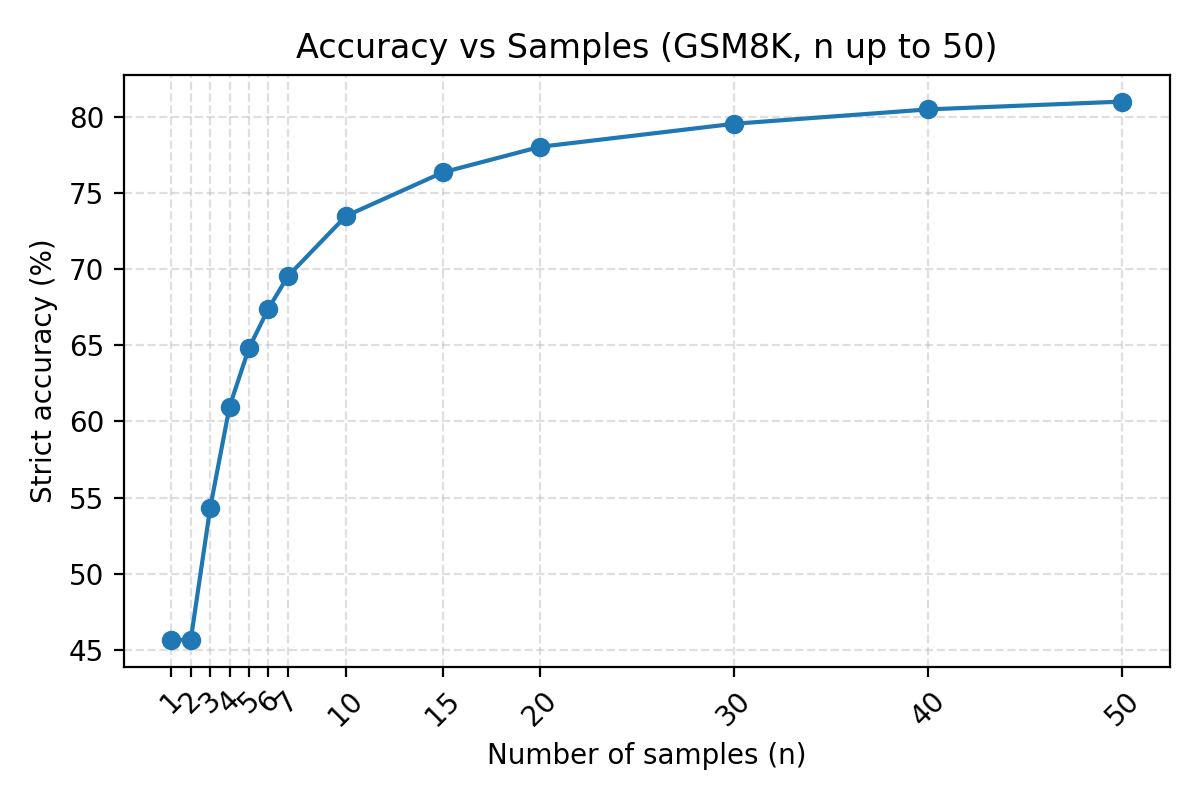
\includegraphics[width=0.8\linewidth]{../../figures/n50_batch/accuracy_vs_n50.png}
  \caption{サンプル数に対する厳密精度の推移}
  \label{fig:accuracy}
\end{figure}

\subsection{初回正解と増分の内訳}
表\ref{tab:first}は初めて正解の多数決を得られたサンプル数の分布である。半数弱(45.7\%)は単一サンプルで正解に到達し,$n=20$ 以降で初めて正解する問題は 401 件に留まる。一方,50 サンプルでも正解しない問題が 1,222 件存在する。

\begin{table}[tb]
  \caption{初回で正解が得られたサンプル数の分布}
  \label{tab:first}
  \centering
  \begin{tabular}{@{}lcc@{}}
    \toprule
    初回正解 $n$ & 件数 & 割合 \\
    \midrule
    1 & 4015 & 45.7\% \\
    3 & 922 & 10.5\% \\
    4 & 657 & 7.5\% \\
    5 & 434 & 4.9\% \\
    7 & 213 & 2.4\% \\
    10 & 368 & 4.2\% \\
    15 & 277 & 3.2\% \\
    20 & 156 & 1.8\% \\
    30 & 124 & 1.4\% \\
    40 & 81 & 0.9\% \\
    50 & 41 & 0.5\% \\
    正解なし & 1222 & 13.9\% \\
    \bottomrule
  \end{tabular}
\end{table}

増分と劣化の件数を図\ref{fig:gain}に示す。$n=2\rightarrow3$ のステップで正解数が最大 (+922 件) 増加し,後半のステップでは純増分が徐々に減るものの $n=40\rightarrow50$ でも +119 件の改善が確認できる。

\begin{figure}[tb]
  \centering
  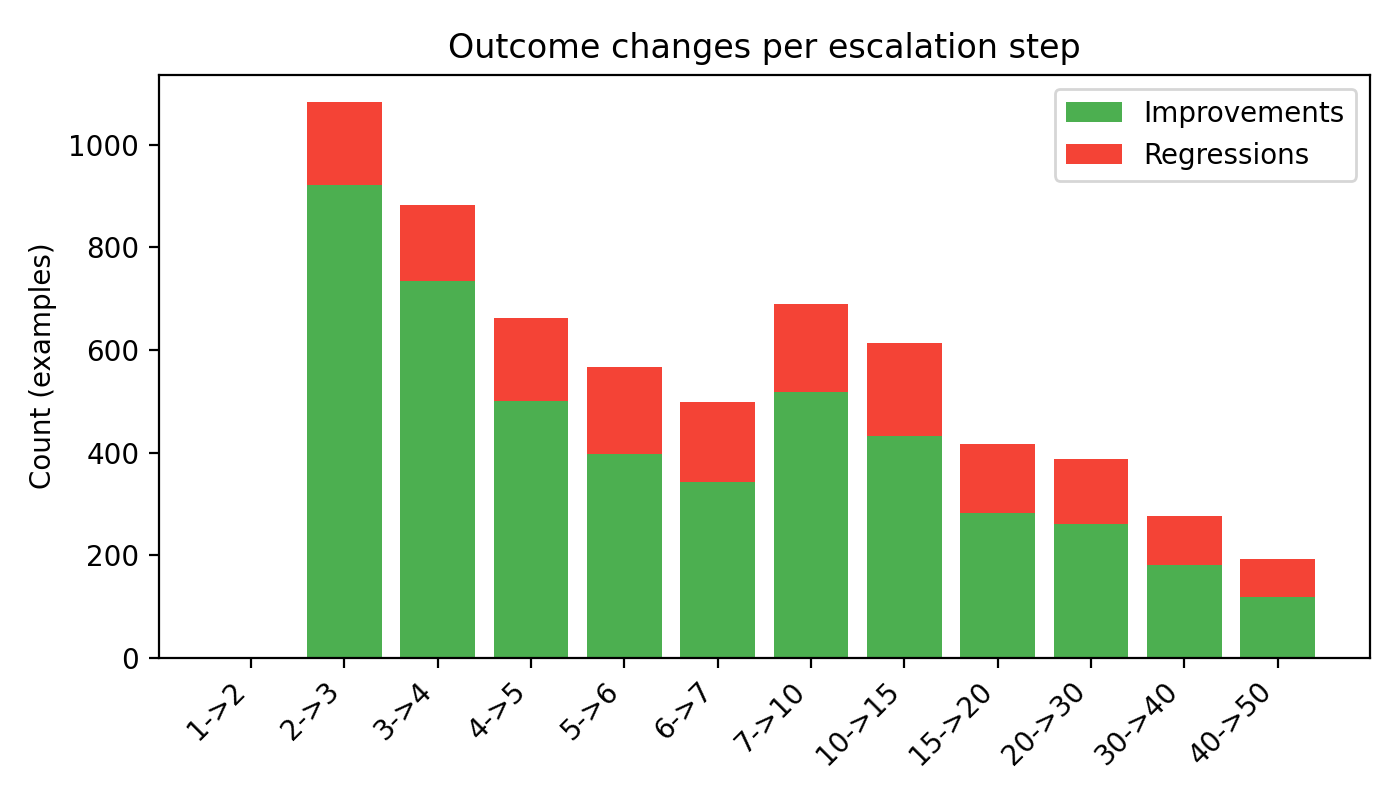
\includegraphics[width=0.95\linewidth]{../../figures/n50_batch/gain_loss_per_step.png}
  \caption{サンプル数拡張ごとの改善件数と劣化件数}
  \label{fig:gain}
\end{figure}

\section{相関分析}
\subsection{全体相関}
投票マージン,二番手票率,プレフィックスエントロピー,レイテンシと正答率/改善量の相関係数を図\ref{fig:corr}に示す。投票マージンは正答率と最も強い正の相関 ($r=0.37$) を持ち,二番手票率は負の相関 ($r=-0.16$) を示した。エントロピーと正答率の相関は $r=0.08$ と弱い。

\begin{figure}[tb]
  \centering
  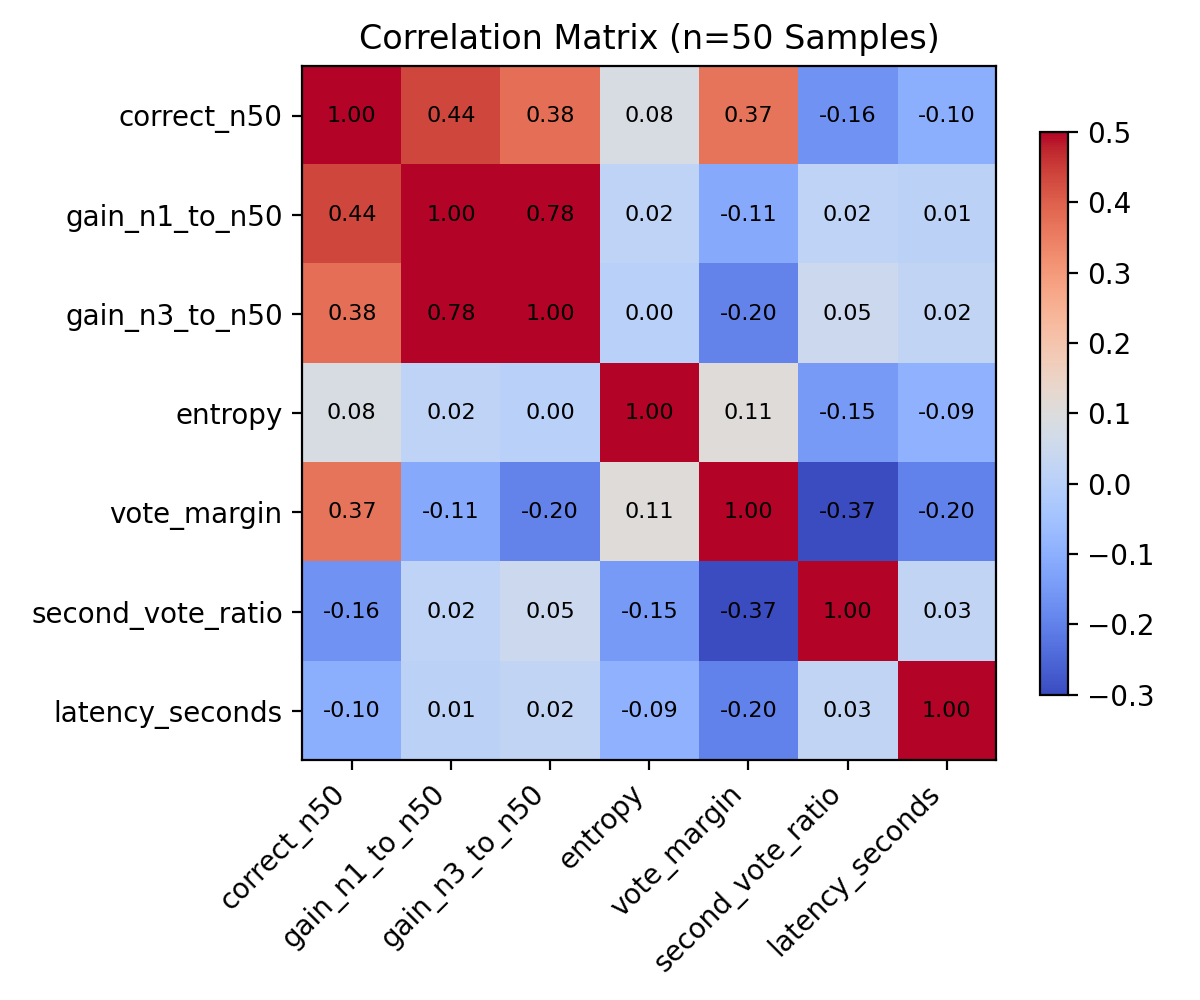
\includegraphics[width=0.95\linewidth]{../../figures/n50_batch/correlation_heatmap.png}
  \caption{正答率・改善量と各特徴量の相関行列}
  \label{fig:corr}
\end{figure}

\subsection{特徴量ごとの精度プロファイル}
投票マージン,エントロピー,二番手票率,レイテンシをビニングした際の精度推移を図\ref{fig:vote}~\ref{fig:latency}に示す。投票マージンが 0.75 を超えると精度は 95\% 以上となり,0.25 未満では 51\% 程度に留まる。二番手票率が 0.40 を超える場合は 60\% を下回るなど,票の競合が失敗の主要因となることが分かった。エントロピーは中間域で高精度を示すが,極端に低いまたは高い領域では緩やかに低下する。レイテンシは 21 秒を超えると 70\% 前後まで落ち込み,時間がかかる問題ほど難易度が高いことが示唆される。

\begin{figure}[tb]
  \centering
  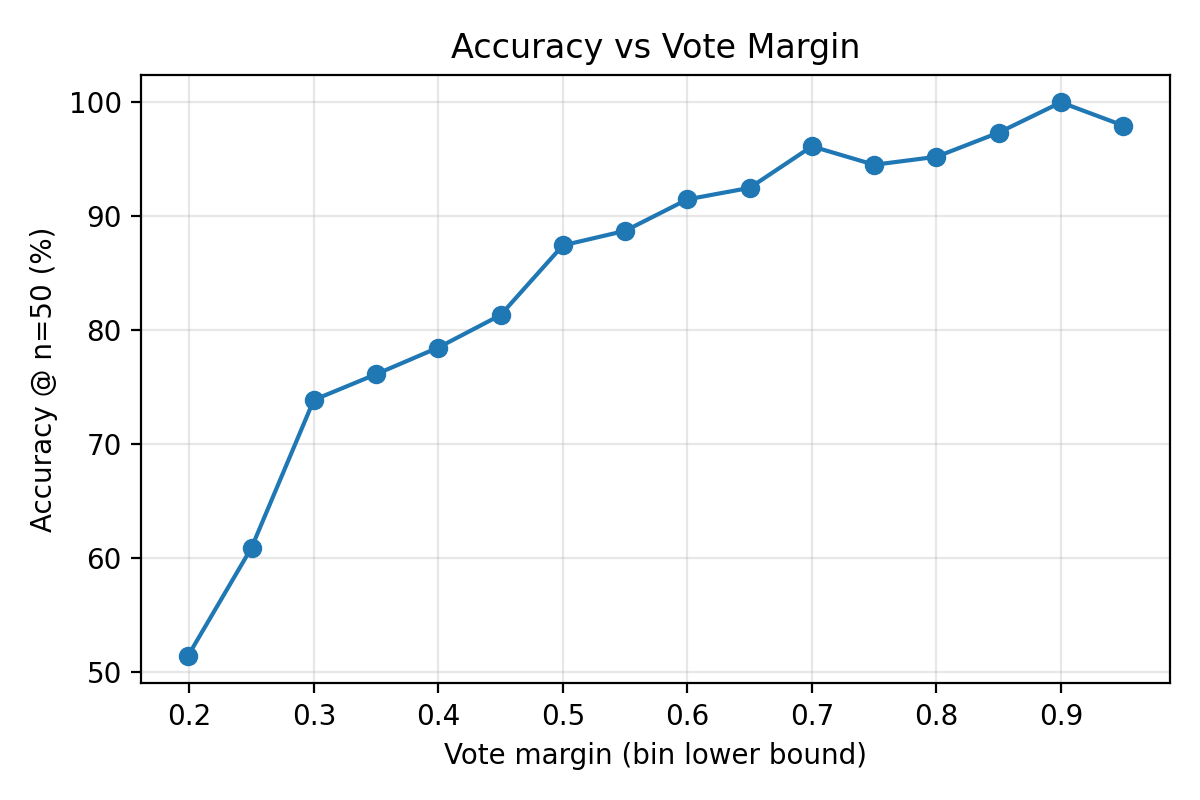
\includegraphics[width=0.8\linewidth]{../../figures/n50_batch/accuracy_vs_vote_margin.png}
  \caption{投票マージン別の精度推移}
  \label{fig:vote}
\end{figure}

\begin{figure}[tb]
  \centering
  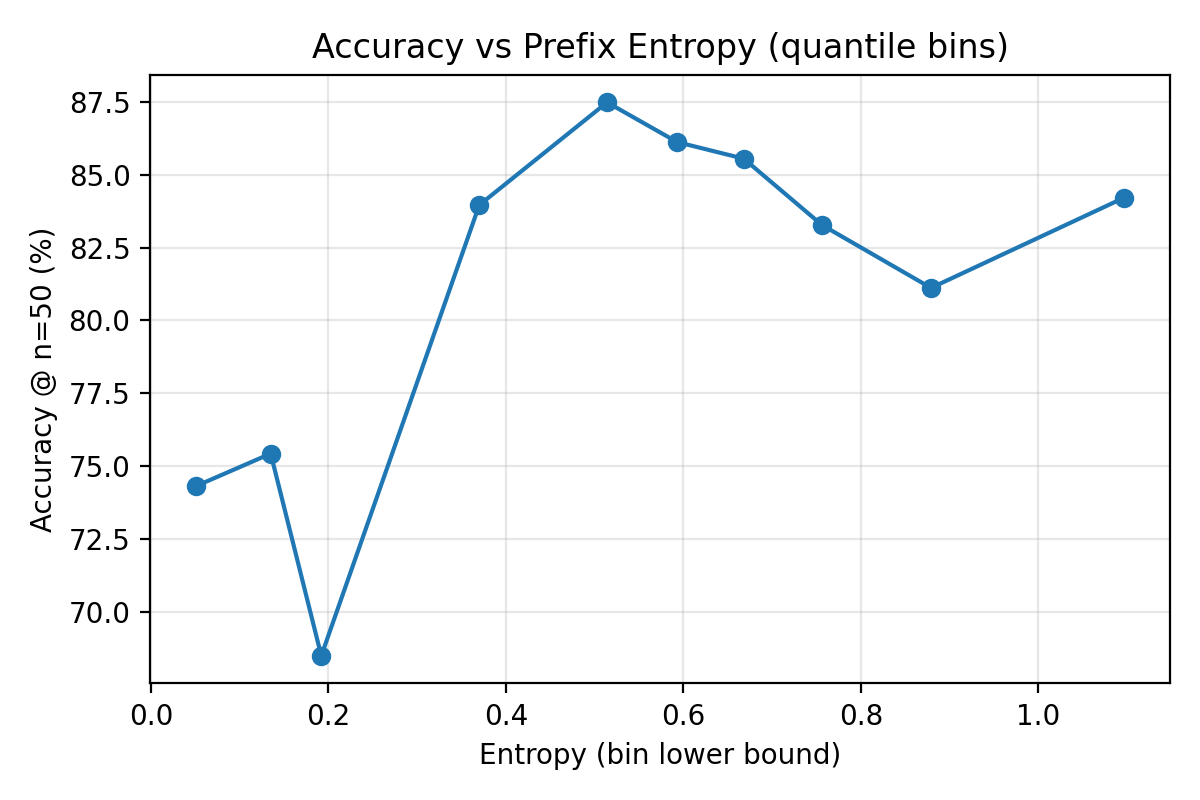
\includegraphics[width=0.8\linewidth]{../../figures/n50_batch/accuracy_vs_entropy.png}
  \caption{プレフィックスエントロピー別の精度推移}
  \label{fig:entropy}
\end{figure}

\begin{figure}[tb]
  \centering
  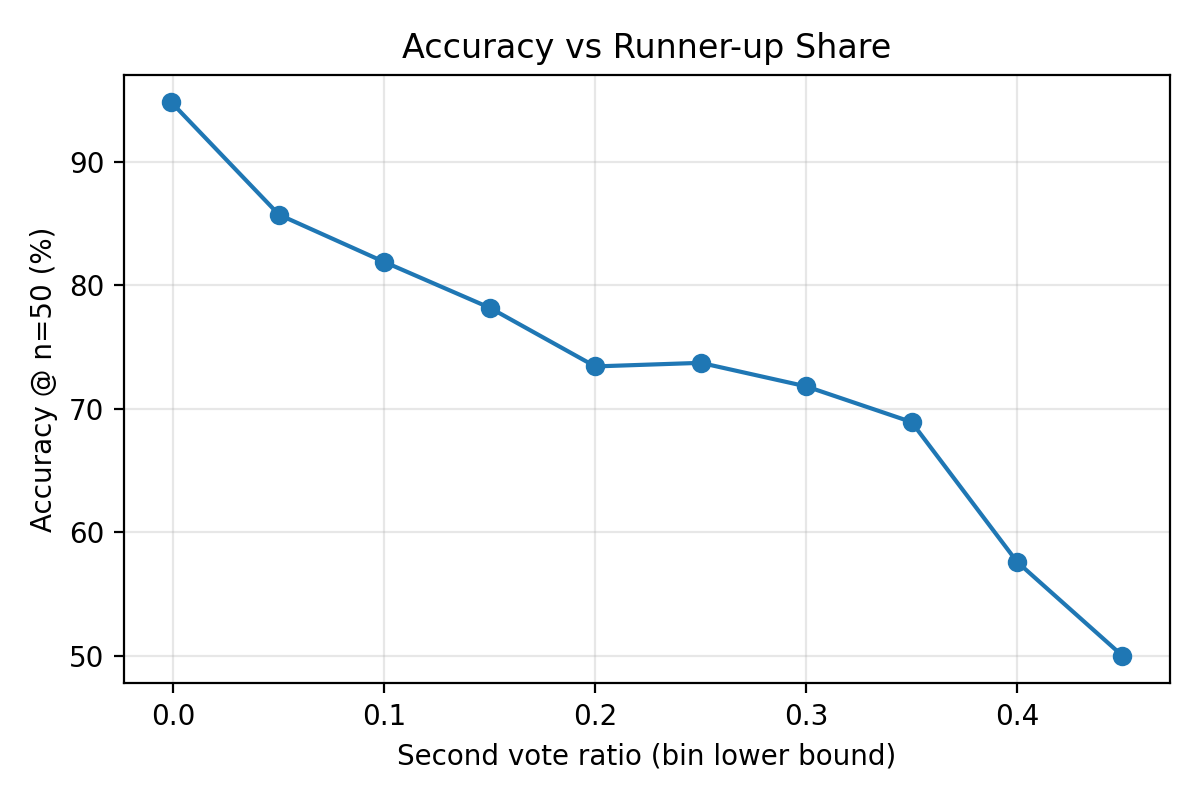
\includegraphics[width=0.8\linewidth]{../../figures/n50_batch/accuracy_vs_second_vote.png}
  \caption{二番手票率別の精度推移}
  \label{fig:second}
\end{figure}

\begin{figure}[tb]
  \centering
  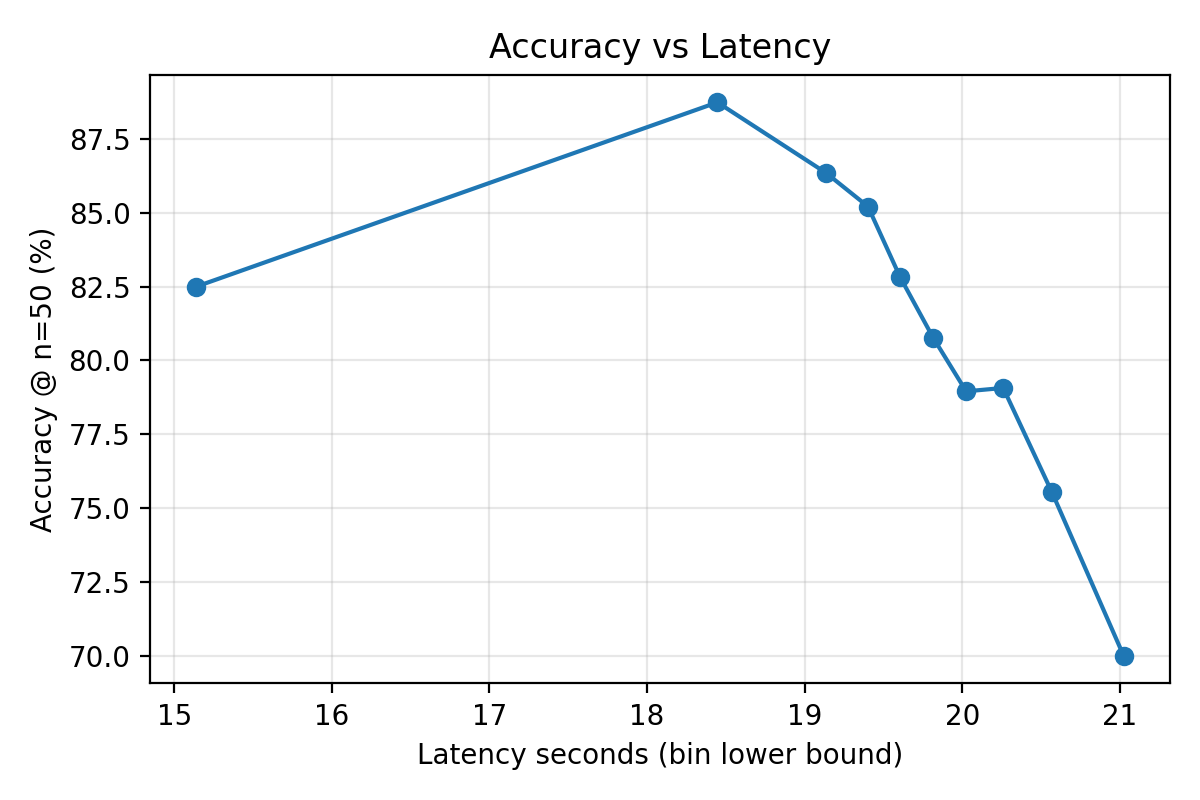
\includegraphics[width=0.8\linewidth]{../../figures/n50_batch/accuracy_vs_latency.png}
  \caption{レイテンシ別の精度推移}
  \label{fig:latency}
\end{figure}

さらに図\ref{fig:scatter}ではエントロピーと投票マージンの散布図を正解ラベルで着色し,高エントロピーでもマージンが十分大きい場合には正答率が保たれることを視覚的に示した。

\begin{figure}[tb]
  \centering
  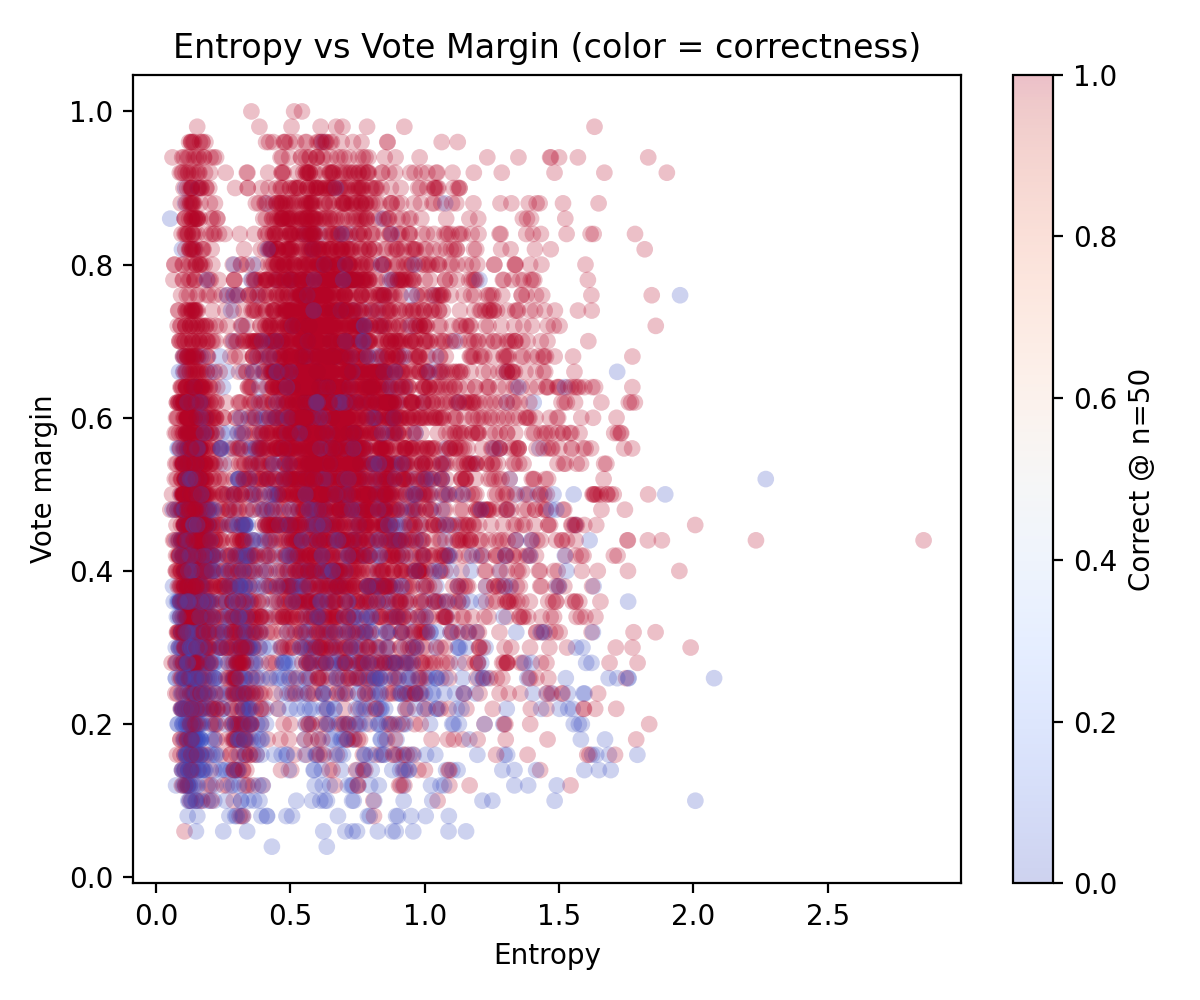
\includegraphics[width=0.85\linewidth]{../../figures/n50_batch/entropy_vs_vote_margin_scatter.png}
  \caption{エントロピーと投票マージンの散布図(色は正誤)}
  \label{fig:scatter}
\end{figure}

\section{考察}
得られた結果から,票の一致度(投票マージンと二番手票率)が信頼性推定の中心的指標であることが確認できた。エントロピーは閾値の粗い決定には利用できるが,単独で難問を識別するには弱い。レイテンシは難問検出の補助指標として有効であり,実運用ではコスト制約と組み合わせたスケジューリングが望ましい。また $n=50$ でも残る 13.9\% の未解決問題には算術ミスや論理破綻が多く見られ,追加の自己検証プロンプトや回答後チェック機構が必要である。

\section{結論と今後の課題}
本報告では CASC-lite の再現実験を $n=50$ まで拡張し,多様な信号と精度との関係を明らかにした。結果として,20 サンプル前後で精度向上が頭打ちになること,投票マージンが最も強い信頼度指標であること,エントロピー単独の識別力は限定的であることが分かった。今後は (1) 投票情報と対数尤度を融合した信頼度モデルの構築,(2) 学習した閾値を用いた前向き実験の実施,(3) 他データセットへの適用を進める予定である。

\section*{謝辞}
CASC-lite の OSS 維持に貢献した開発者に感謝する。

\begin{thebibliography}{9}
\bibitem{original-report} CASC-lite repository documentation, \\ \url{https://github.com/your-org/casc-lite-entropy-adaptive-sc}
\bibitem{gsm8k} Cobbe, K. et al., GSM8K: A dataset for grade school math word problems, arXiv:2110.14168, 2021.
\end{thebibliography}

\end{document}
